\subsection{Аналоги программного средства}

\subsubsection{Сервис для управления бизнесом \analogBitrics}

Одна из наиболее широко распространенных реализаций будущего программного средства является сервис для управления
бизнесом \analogBitrics.

Многофункциональная платформа для управления бизнесом, включающая CRM, задачи, чаты, телефонию, документы и
автоматизацию процессов. Пользователь получает доступ к единому рабочему пространству, где можно вести базу
клиентов, управлять сделками, общаться с коллегами и контролировать задачи. Интерфейс ориентирован на обычного
пользователя без технических знаний, с возможностью гибко настраивать воронки продаж, автоматизировать действия
и интегрироваться с популярными сервисами (почта, мессенджеры, телефония).

Рассмотреть данный сервис можно на рисунке \ref{fig:bitrics}.

\begin{figure}[ht]
    \centering
    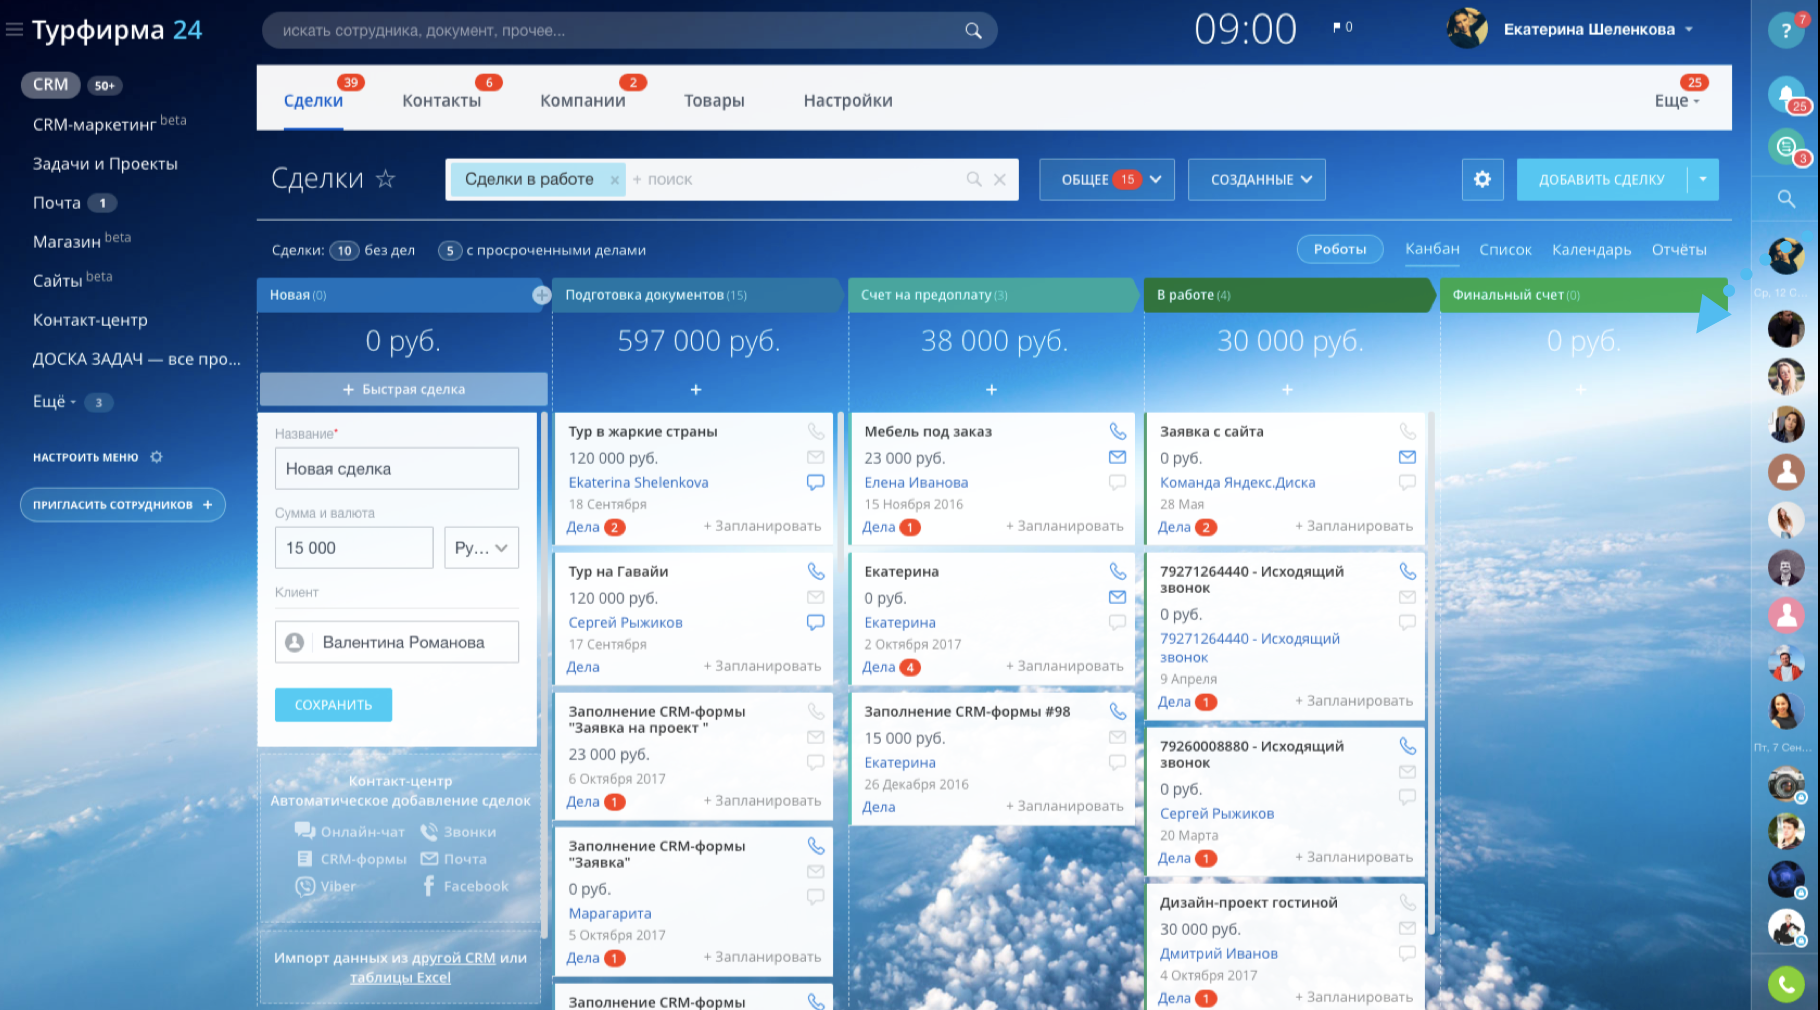
\includegraphics[width=0.65\linewidth]{\commonSecPathPrefix/sec_1/content/bitrics.png}
    \caption{Программное средство \analogBitrics}
    \label{fig:bitrics}
\end{figure}

К преимуществам системы можно отнести богатый функционал в базовой версии продукта, наличие бесплатного тарифа, облачную 
версию, доступ с мобильных устройств и широкие возможности автоматизации. Минусы — перегруженность интерфейса, особенно для
новых пользователей, ограниченная гибкость на бесплатном тарифе, а также заметное снижение скорости работы при большом
объеме данных или использовании коробочной версии без оптимизации.

\subsubsection{Программное средство \analogZoho}

Ещё одной реализацией является программное средство \analogZoho.

{\analogZoho} — это облачная CRM-система, ориентированная на автоматизацию продаж, маркетинга и клиентского сервиса. 
Пользователь работает в чистом и понятном интерфейсе, где легко отслеживать взаимодействие с клиентами, управлять лидами, 
сделками и задачами. Система предлагает гибкую настройку воронок продаж, автоматические сценарии, аналитику и интеграции с 
другими продуктами Zoho и внешними сервисами, включая почту, мессенджеры и соцсети.

Интерфейс программного средства представлен на рисунке \ref{fig:zoho}.

\begin{figure}[ht]
    \centering
    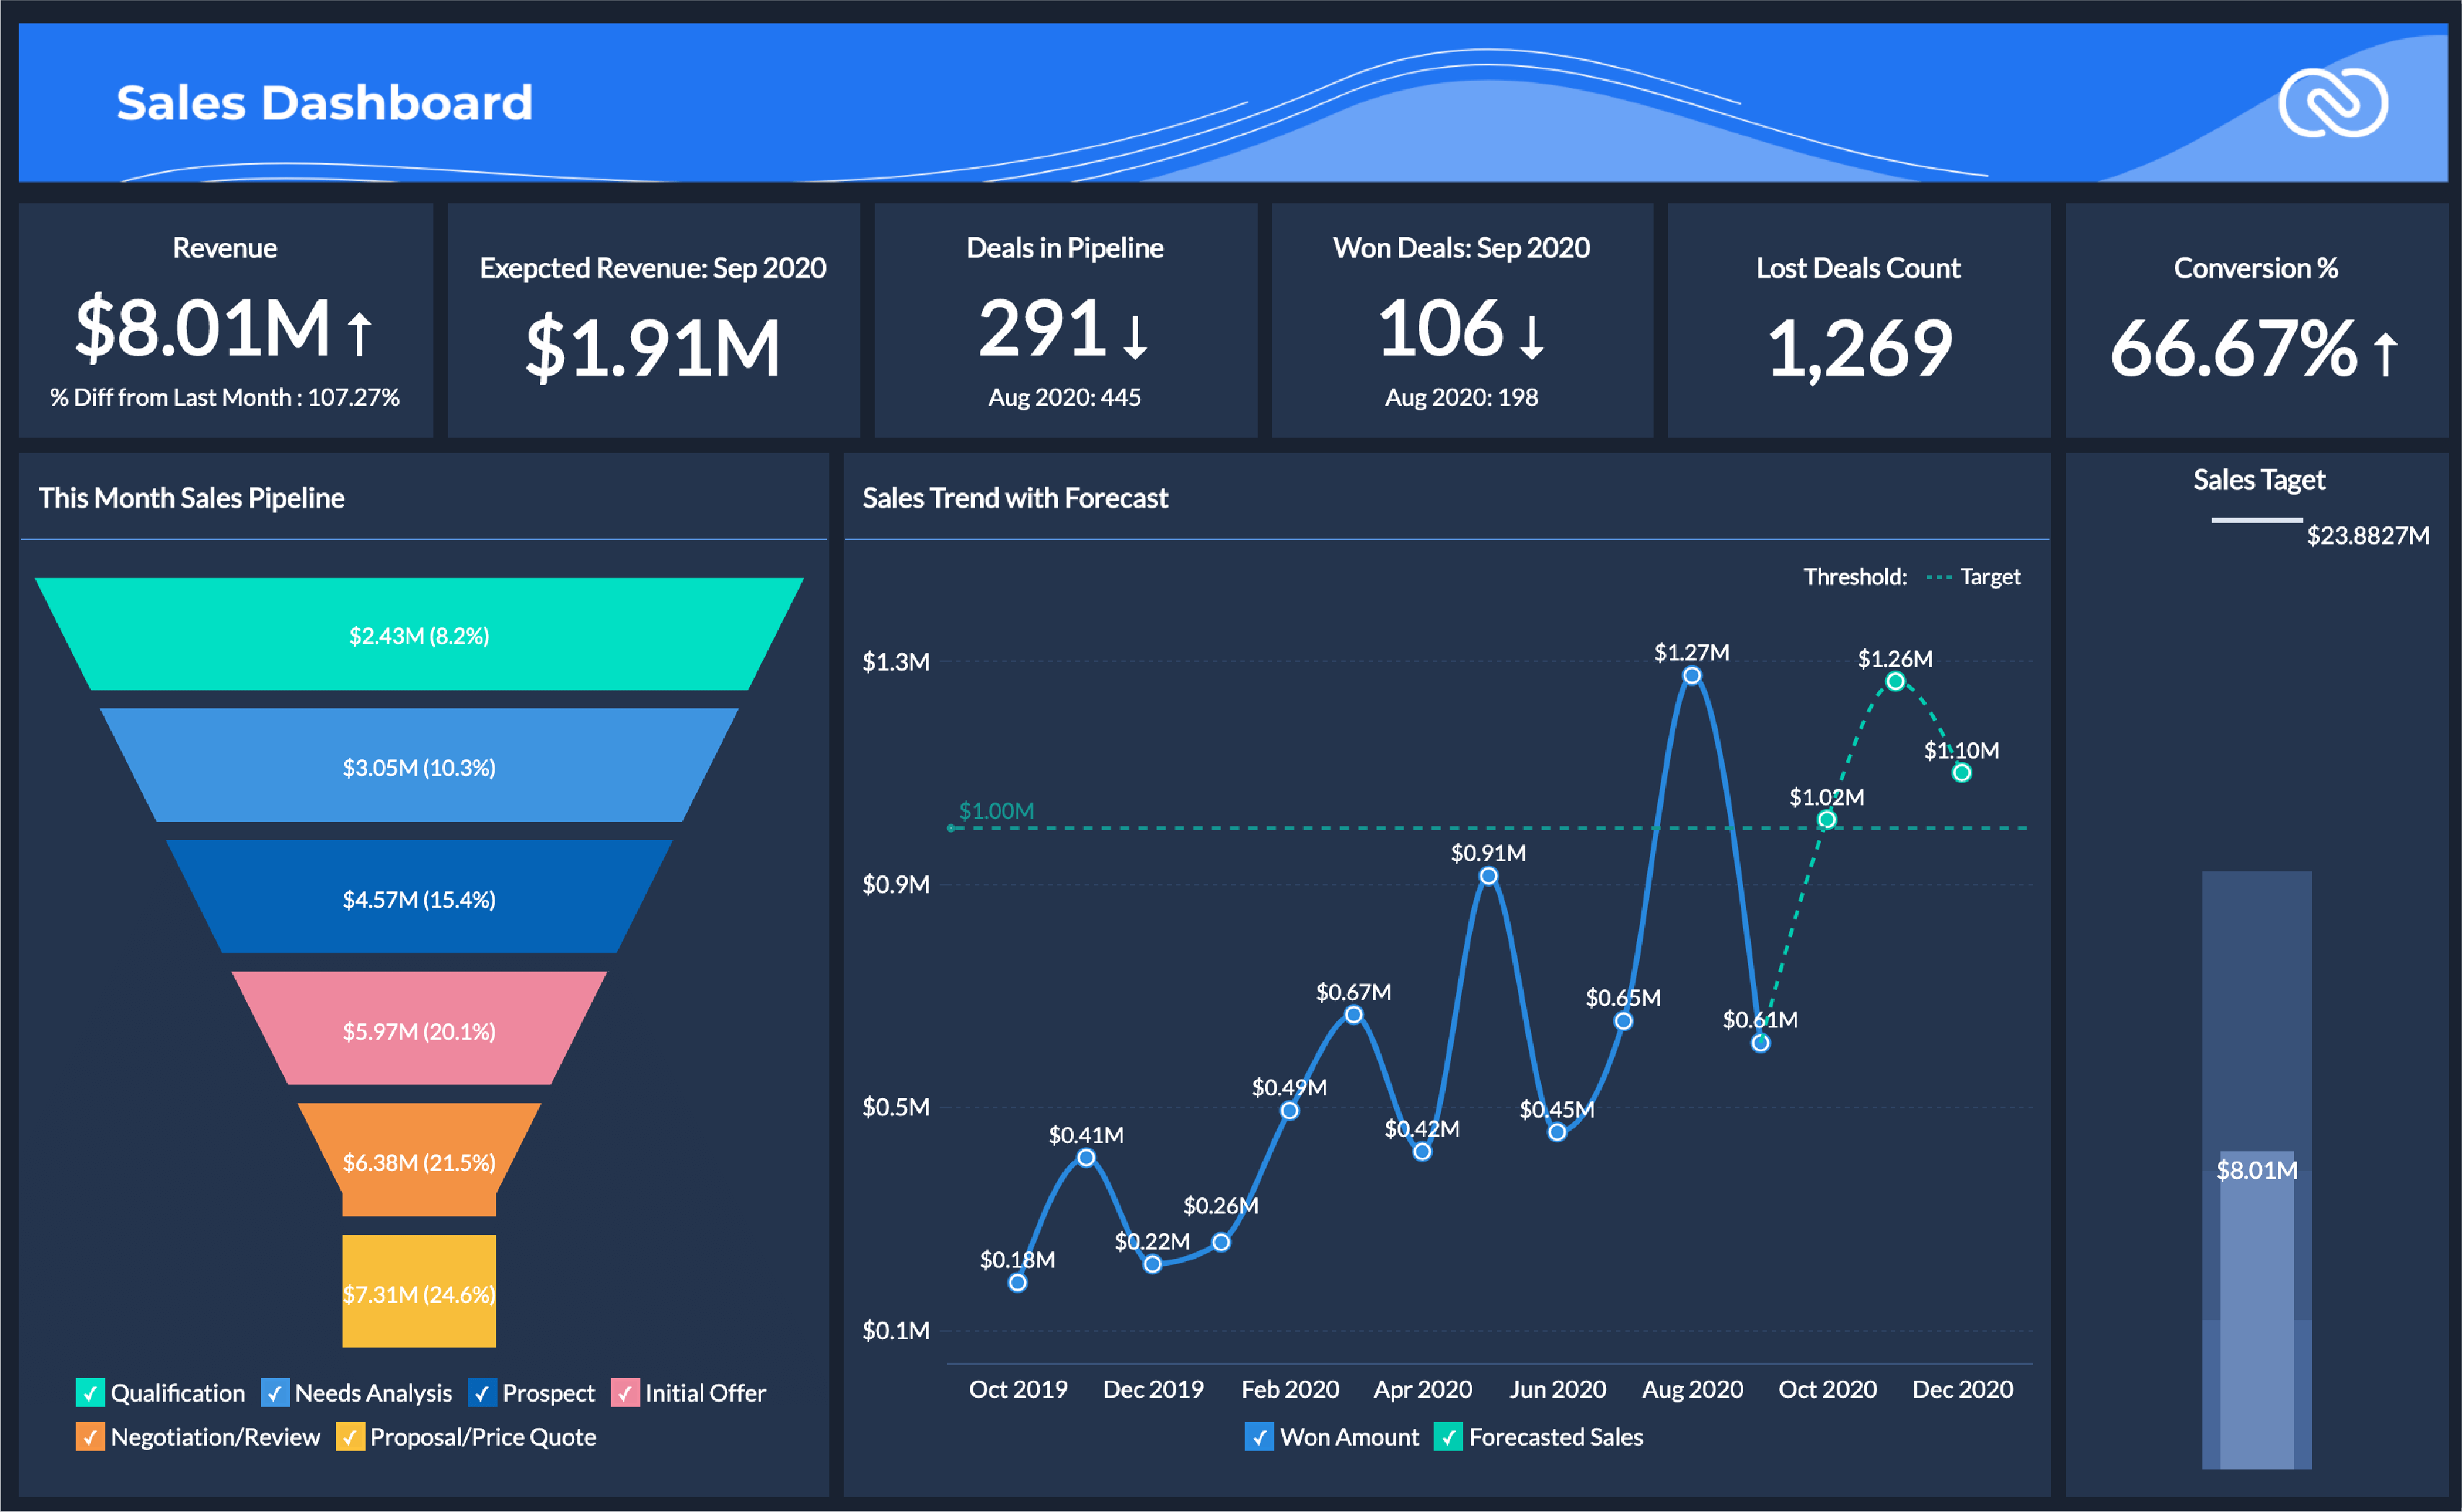
\includegraphics[width=0.65\linewidth]{\commonSecPathPrefix/sec_1/content/zoho.png}
    \caption{Программное средство \analogZoho}
    \label{fig:zoho}
\end{figure}

\subsubsection{Система взаимоотношений \analogOneC}

Одним из наиболее популярных и широко используемых программных решений для управления взаимоотношениями с клиентами на 
рынке является {\analogOneC} — специализированный модуль в составе платформы \analogOneCMain. Это программное средство ориентировано 
на автоматизацию процессов взаимодействия с клиентами и партнёрами, управление продажами, маркетингом и сервисным обслуживанием. 
Оно предназначено для использования как в малом и среднем бизнесе, так и в крупных организациях с развитой системой клиентских 
коммуникаций.

Рассмотреть данный сервис можно на рисунке \ref{fig:onec}.

\begin{figure}[ht]
    \centering
    \fbox{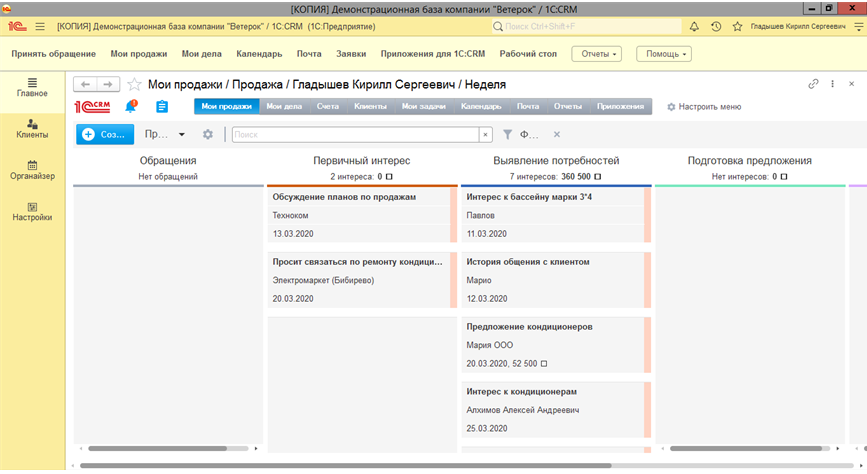
\includegraphics[width=0.65\linewidth]{\commonSecPathPrefix/sec_1/content/onec.png}}
    \caption{Программное средство \analogOneC}
    \label{fig:onec}
\end{figure}

{\analogOneC} обеспечивает централизованное хранение информации о клиентах, историях взаимодействий, сделках, заявках, контактах и других
аспектах делового общения. Система позволяет вести учёт и планирование задач, контролировать исполнение поручений, сегментировать
клиентскую базу, анализировать эффективность маркетинговых мероприятий и прогнозировать продажи.

Система гибко настраивается под нужды конкретной компании и интегрируется с другими продуктами линейки 1С, а также с внешними сервисами 
(например, почтовыми клиентами, IP-телефонией и сайтами).